\documentclass[main]{subfiles}

\begin{document}

\section{Empirical Results}\label{sec:results}
In this section, we consider real data examples to compare the performances of different flavors of UACP, with different number of sources and different sizes of the sources. We consider seven different scenarios for the number and size of the data sources, we call them different methods.  We apply these different methods to five real datasets. For each dataset, we split the data into ten folds, where each fold consists of a training set and an independent test set.Then we apply these different methods to all ten folds of each five real datasets. In order to compare the various methods, we look at the two performance measures validity (\ref{eq:validity}) and efficiency (\ref{eq:efficiency}). %All reported results are based on application of different methods to all ten folds of each five real datasets. 

For each dataset we consider the following configurations:

\begin{enumerate}

\item Given a dataset, we split the data into ten folds, where each fold consists of a training set (80\%) and an independent test set (20\%).

\item for each folds we split the training dataset into various number of sources, as follow:
\begin{enumerate}
	\item Single source or pooled data  where training set is considered as a single source.
	\item Equal sized sources: training set is randomly partitioned into equal sized sources and  each partition is considered as a proper training set to model and compute p-values, and then p-values are aggregated for all sources. We mainly consider 2, 4 and 6 equal sized sources. %in three different settings.
	\item Unequal sized sources: training set is randomly partitioned into unequal sized sources and  each partition is considered as a proper training set to model and compute p-values, and then p-values are aggregated for all sources. We mainly consider 2, 4 and 6 unequal sized sources, and we repeat it five times to get five different set of sizes for each source.

\end{enumerate}

\end{enumerate}

Repeat the step 1 and step 2 with five different datasets, and combine the results for each method. Then paiwise compare the validity and efficiency for all methods. %Single source, 2EqualSizedSource, 4EqualSizedSource, 6EqualSizedSource, 2UnequalSizedSource, 4UnequalSizedSource and 6UnequalSizedSource. The details of the datasets used and the results on individual datasets are given in Supplementary Material.%are given in the following, these data have been taken from the UCI Repository of machine learning batabases: ftp://ftp.ics.uci.edu/pub/machine-learning-databases/.


%\subsection{Empirical results on Combined data}
The results for comparing the different methods on combined results, by applying the Wilcoxon signed-rank test on validity and efficiency are shown in Figure \ref{fig:testCombined}. To quantify the difference between various methods the box plots are given in Figure \ref{fig:boxplotCombined}.

\begin{figure}[H]
\centering
\begin{subfigure}{\textwidth}
  \centering
  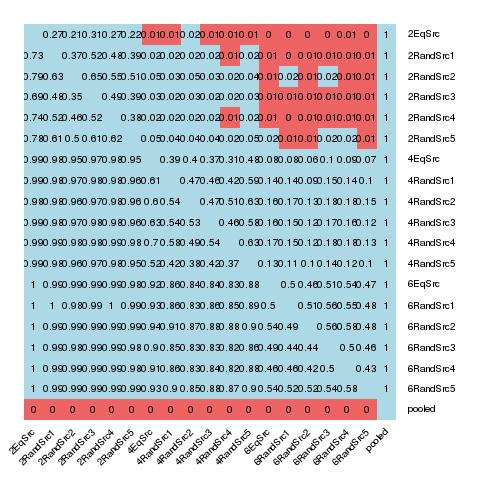
\includegraphics[width=.75\linewidth]{images/heatmapCombined}
%  \caption{Validity}  \label{fig:valCombined}
\end{subfigure}%

\begin{subfigure}{\textwidth}
  \centering
  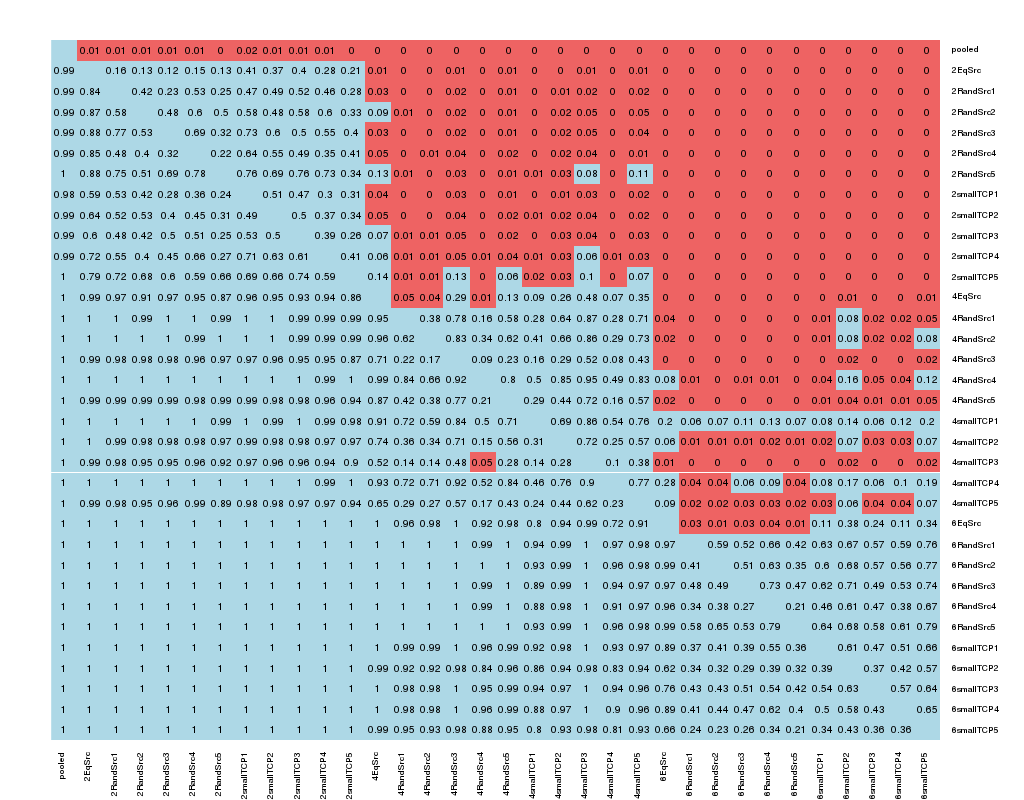
\includegraphics[width=.75\linewidth]{images/heatmapCombined_eff}
  %\caption{Efficiency}  \label{fig:effCombined}
\end{subfigure}%
\caption{Results of Wilcoxon signed-rank tests for two alterna-
tive hypotheses relating validity (a) and observed fuzziness (b) with combining all the datasets. The p-values are shown for the methods in the right column having greater values than the methods in the first row. All significant p-values are marked in red.} \label{fig:testCombined}
\end{figure}

 \begin{figure}[H]
\centering
\begin{subfigure}{\textwidth}\centering
  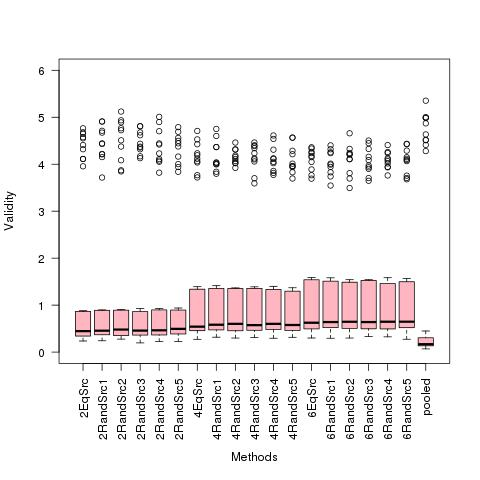
\includegraphics[width=12cm,height=6cm]{images/boxplotCombined}
%  \caption{Validity}  \label{fig:valBC}
\end{subfigure}%

\begin{subfigure}{\textwidth} \centering
 
  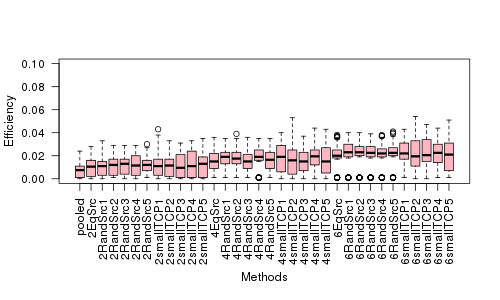
\includegraphics[width=12cm,height=6cm]{images/boxplotCombined_eff}
 % \caption{Efficiency}  \label{fig:effBC}
\end{subfigure}%
\caption{Box plot of validity (a) and observed fuzziness (b) with combined data.} \label{fig:boxplotCombined}
\end{figure}



\section{Conclusions}
We propose to aggregate conformal predictions from multiple sources and apply it to the various real life classification datasets. The  method  is  a  straightforward
generalization of the basic conformal prediction framework to handle multiple data sources that do not require sharing of data. %Our  analysis presents 

\end{document}
